\documentclass[journal]{IEEEtran}

% *** CITATION PACKAGES ***
%
%\usepackage{cite}
\usepackage{capt-of}%%To get the caption
\usepackage{gensymb}
\usepackage{graphicx} %package to manage images
\graphicspath{ {./images/} }
\usepackage{wrapfig}

\usepackage[style=ieee]{biblatex}
\DeclareLanguageMapping{english}{english-apa}
\addbibresource{references.bib}
\usepackage[justification=centering]{caption}

\usepackage{setspace}

\usepackage{hhline}

\usepackage{booktabs}

% *** GRAPHICS RELATED PACKAGES ***
%
\ifCLASSINFOpdf
  % \usepackage[pdftex]{graphicx}
  % declare the path(s) where your graphic files are
  % \graphicspath{{../pdf/}{../jpeg/}}
  % and their extensions so you won't have to specify these with
  % every instance of \includegraphics
  % \DeclareGraphicsExtensions{.pdf,.jpeg,.png}
\else
  % or other class option (dvipsone, dvipdf, if not using dvips). graphicx
  % will default to the driver specified in the system graphics.cfg if no
  % driver is specified.
  % \usepackage[dvips]{graphicx}
  % declare the path(s) where your graphic files are
  % \graphicspath{{../eps/}}
  % and their extensions so you won't have to specify these with
  % every instance of \includegraphics
  % \DeclareGraphicsExtensions{.eps}
\fi
% graphicx was written by David Carlisle and Sebastian Rahtz. It is
% required if you want graphics, photos, etc. graphicx.sty is already
% installed on most LaTeX systems. The latest version and documentation
% can be obtained at: 
% http://www.ctan.org/pkg/graphicx
% Another good source of documentation is "Using Imported Graphics in
% LaTeX2e" by Keith Reckdahl which can be found at:
% http://www.ctan.org/pkg/epslatex
%
% latex, and pdflatex in dvi mode, support graphics in encapsulated
% postscript (.eps) format. pdflatex in pdf mode supports graphics
% in .pdf, .jpeg, .png and .mps (metapost) formats. Users should ensure
% that all non-photo figures use a vector format (.eps, .pdf, .mps) and
% not a bitmapped formats (.jpeg, .png). The IEEE frowns on bitmapped formats
% which can result in "jaggedy"/blurry rendering of lines and letters as
% well as large increases in file sizes.
%
% You can find documentation about the pdfTeX application at:
% http://www.tug.org/applications/pdftex

\begin{document}

\begin{titlepage}
    {\centering
        \vspace*{20em}
        {
        \huge 
        \begin{spacing}{1.5}
            Lab Report \#4 
            \\
            Circuits Fundamentals Lab, Spring 2019
            \bigskip
            \Large
            \\
            Determining the Capacitance of a Built Capacitor\\
            By Analysis of a Low Pass and High Pass Filter
  
            \\
            \bigskip
            Deadline: March 3, 2019 
        \end{spacing}

        }
        
    }
    \vfill
    
    {
    \large
    
    \begin{spacing}{1.5}
    \noindent Barkin Simsek, {\it {bs3528@nyu.edu}} 
    \\
    Nishant Aswani, {\it {nsa325@nyu.edu}}
    \\
    Section \#1% <-this % stops a space
    \\
    Workstation \#8% <-this % stops a space
    \end{spacing}
    }


\end{titlepage}
\pagenumbering{gobble}
%\clearpage\mbox{} % adds and empty page
%\clearpage
\pagenumbering{arabic}
\setcounter{page}{1}

%\title{Demonstration of a Voltage Divider With A Variable Resistor}

%\author{Barkin Simsek,~\IEEEmembership{bs3528@nyu.edu};
%Nishant Aswani,~\IEEEmembership{nsa325@nyu.edu}
%\\ Table Number: \#}% <-this % stops a space


% The paper headers
\markboth{Simsek, Aswani, Circuits Fundamentals Lab 2019}%
{}

% make the title area
%\maketitle

% As a general rule, do not put math, special symbols or citations
% in the abstract or keywords.
\begin{abstract}
In this experiment, a variable capacitor was built by using aluminum foil, A4 paper, and a PVC pipe. The capacitor was used to implement a high and low pass filter, through which AC signals were passed at varying frequencies and the output was measured using an oscilloscope, thus allowing for the calculation of the capacitance. The high pass filter led to a maximum capacitance of 0.88 nF, while the low pass filter led to a maximum capacitance of 0.76 nF, compared to the measured max. capacitance of 0.82 nF. Further, low pass filter led to a minimum capacitance of 0.46 nF, compared to a calculated capacitance of 0.33 nF.
\end{abstract}






%Percenta of power being consumed at the internal resistence

%What happens to voltage when external load is connected and current %consumption increaased

%Formula derivation
%Application 


\section{Introduction}
\IEEEPARstart{T}\lowercase{he} purpose of this lab was to produce a variable capacitor and connect it to a low-pass and high-pass filter circuit. In connecting the capacitor to the above-mentioned circuits, the goal was to experimentally obtain the maximum and minimum capacitance of the capacitor.\\

\noindent Capacitors are essentially two conductive plates, often with a dielectric material in between, which serves the purpose of reducing the electric field strength and thus increasing capacitance. Reducing the electric field strength has the effect of reducing the voltage; storing charge at a lower voltage increases the capacitance of the capacitor (see Equation \ref{eq:cap}).

\begin{equation}
C \propto \frac{1}{E}
\label{eq:cap}
\end{equation}

\noindent In direct current (DC) circuits, capacitors are used as "storage devices" to collect charge as long as a voltage is constantly applied. On the other hand, in alternating current (AC) circuits, the capacitor charges and discharges as the current alternates. This charging and discharging behavior occurs in a 90\degree  phase difference to the alternating current. Due to different behavior based on either DC or AC, capacitors are often used in high pass (HPF) and low pass filters (LPF) to filter out certain signals. The placement of capacitors in HPF and LPF is shown in Figures \ref{fig:HPF} and \ref{fig:LPF}.

\begingroup
    \centering
    %width=\columnwidth
    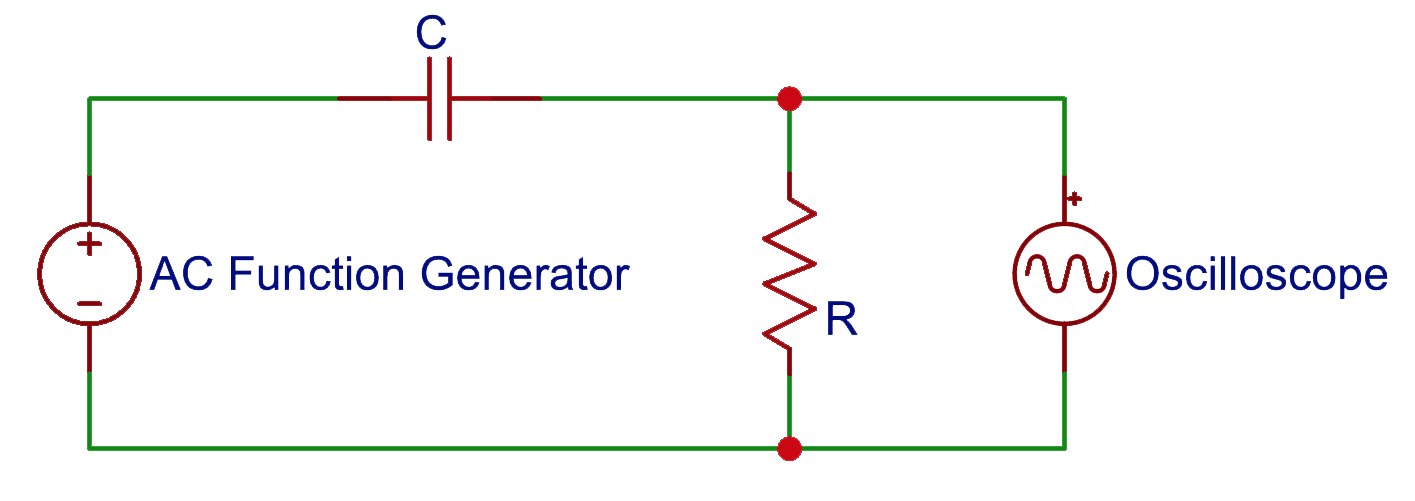
\includegraphics[width=245]{images/lab4_6.png}
    \captionof{figure}{A high-pass filter. For example, in a microphone, capacitors are placed in series with the mix of DC (power) and AC (sound) input signals to filter out or block the low-frequency DC and pass the high-frequency AC.}
    \label{fig:HPF}
\endgroup

\begingroup
    \centering
    %width=\columnwidth
    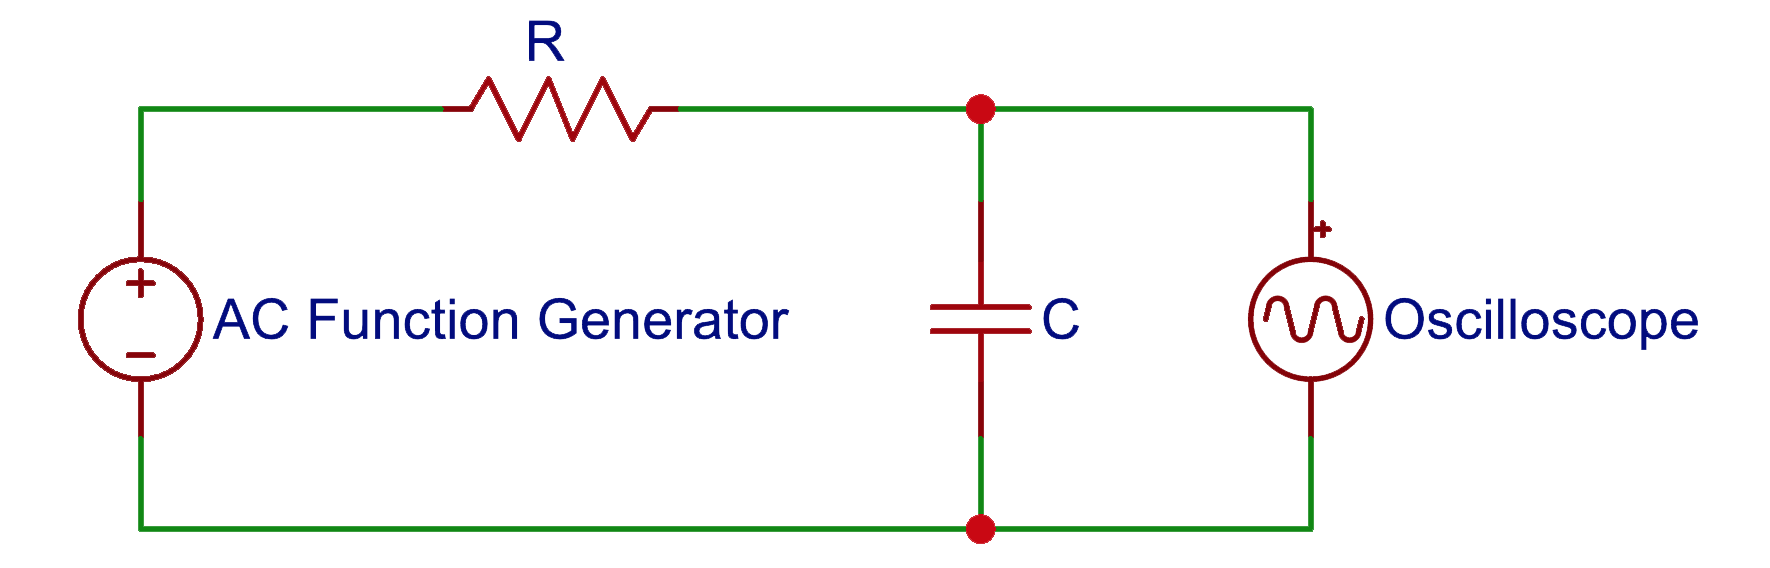
\includegraphics[width=245]{images/lab4_5.png}
    \captionof{figure}{A low-pass filter. The high-frequency signals pass through the capacitor and thus only low-frequency signals are recorded.}
    \label{fig:LPF}
\endgroup

\section{Building the Capacitor}

\noindent A capacitor can be made variable by varying the effective area of the plates or distance between conductive plates. Thus, this lab used two pieces aluminum foil with a piece of paper in between. It was designed so that the the top piece of aluminum was capable of sliding up or down the bottom piece to increase or decrease the area and thus the capacitance. \\

\noindent A piece of aluminum foil, slightly smaller than the size of an A4 paper, was taped to an A4 paper. One end of a multi-core wire was stripped and spread out across the aluminium piece to increase surface area, completing the first component. This process was repeated to produce an identical second component. The first component was wrapped around a PVC pipe, with the aluminum facing the inside. The second component was loosely taped around the first piece, with the aluminum facing inwards. As a result, a variable capacitor was made, shown in Figures \ref{fig:mincap} and \ref{fig:maxcap}. The two black cables running act as the two terminals of the capacitor.

\begingroup
    \medskip
    \centering
    %width=\columnwidth
    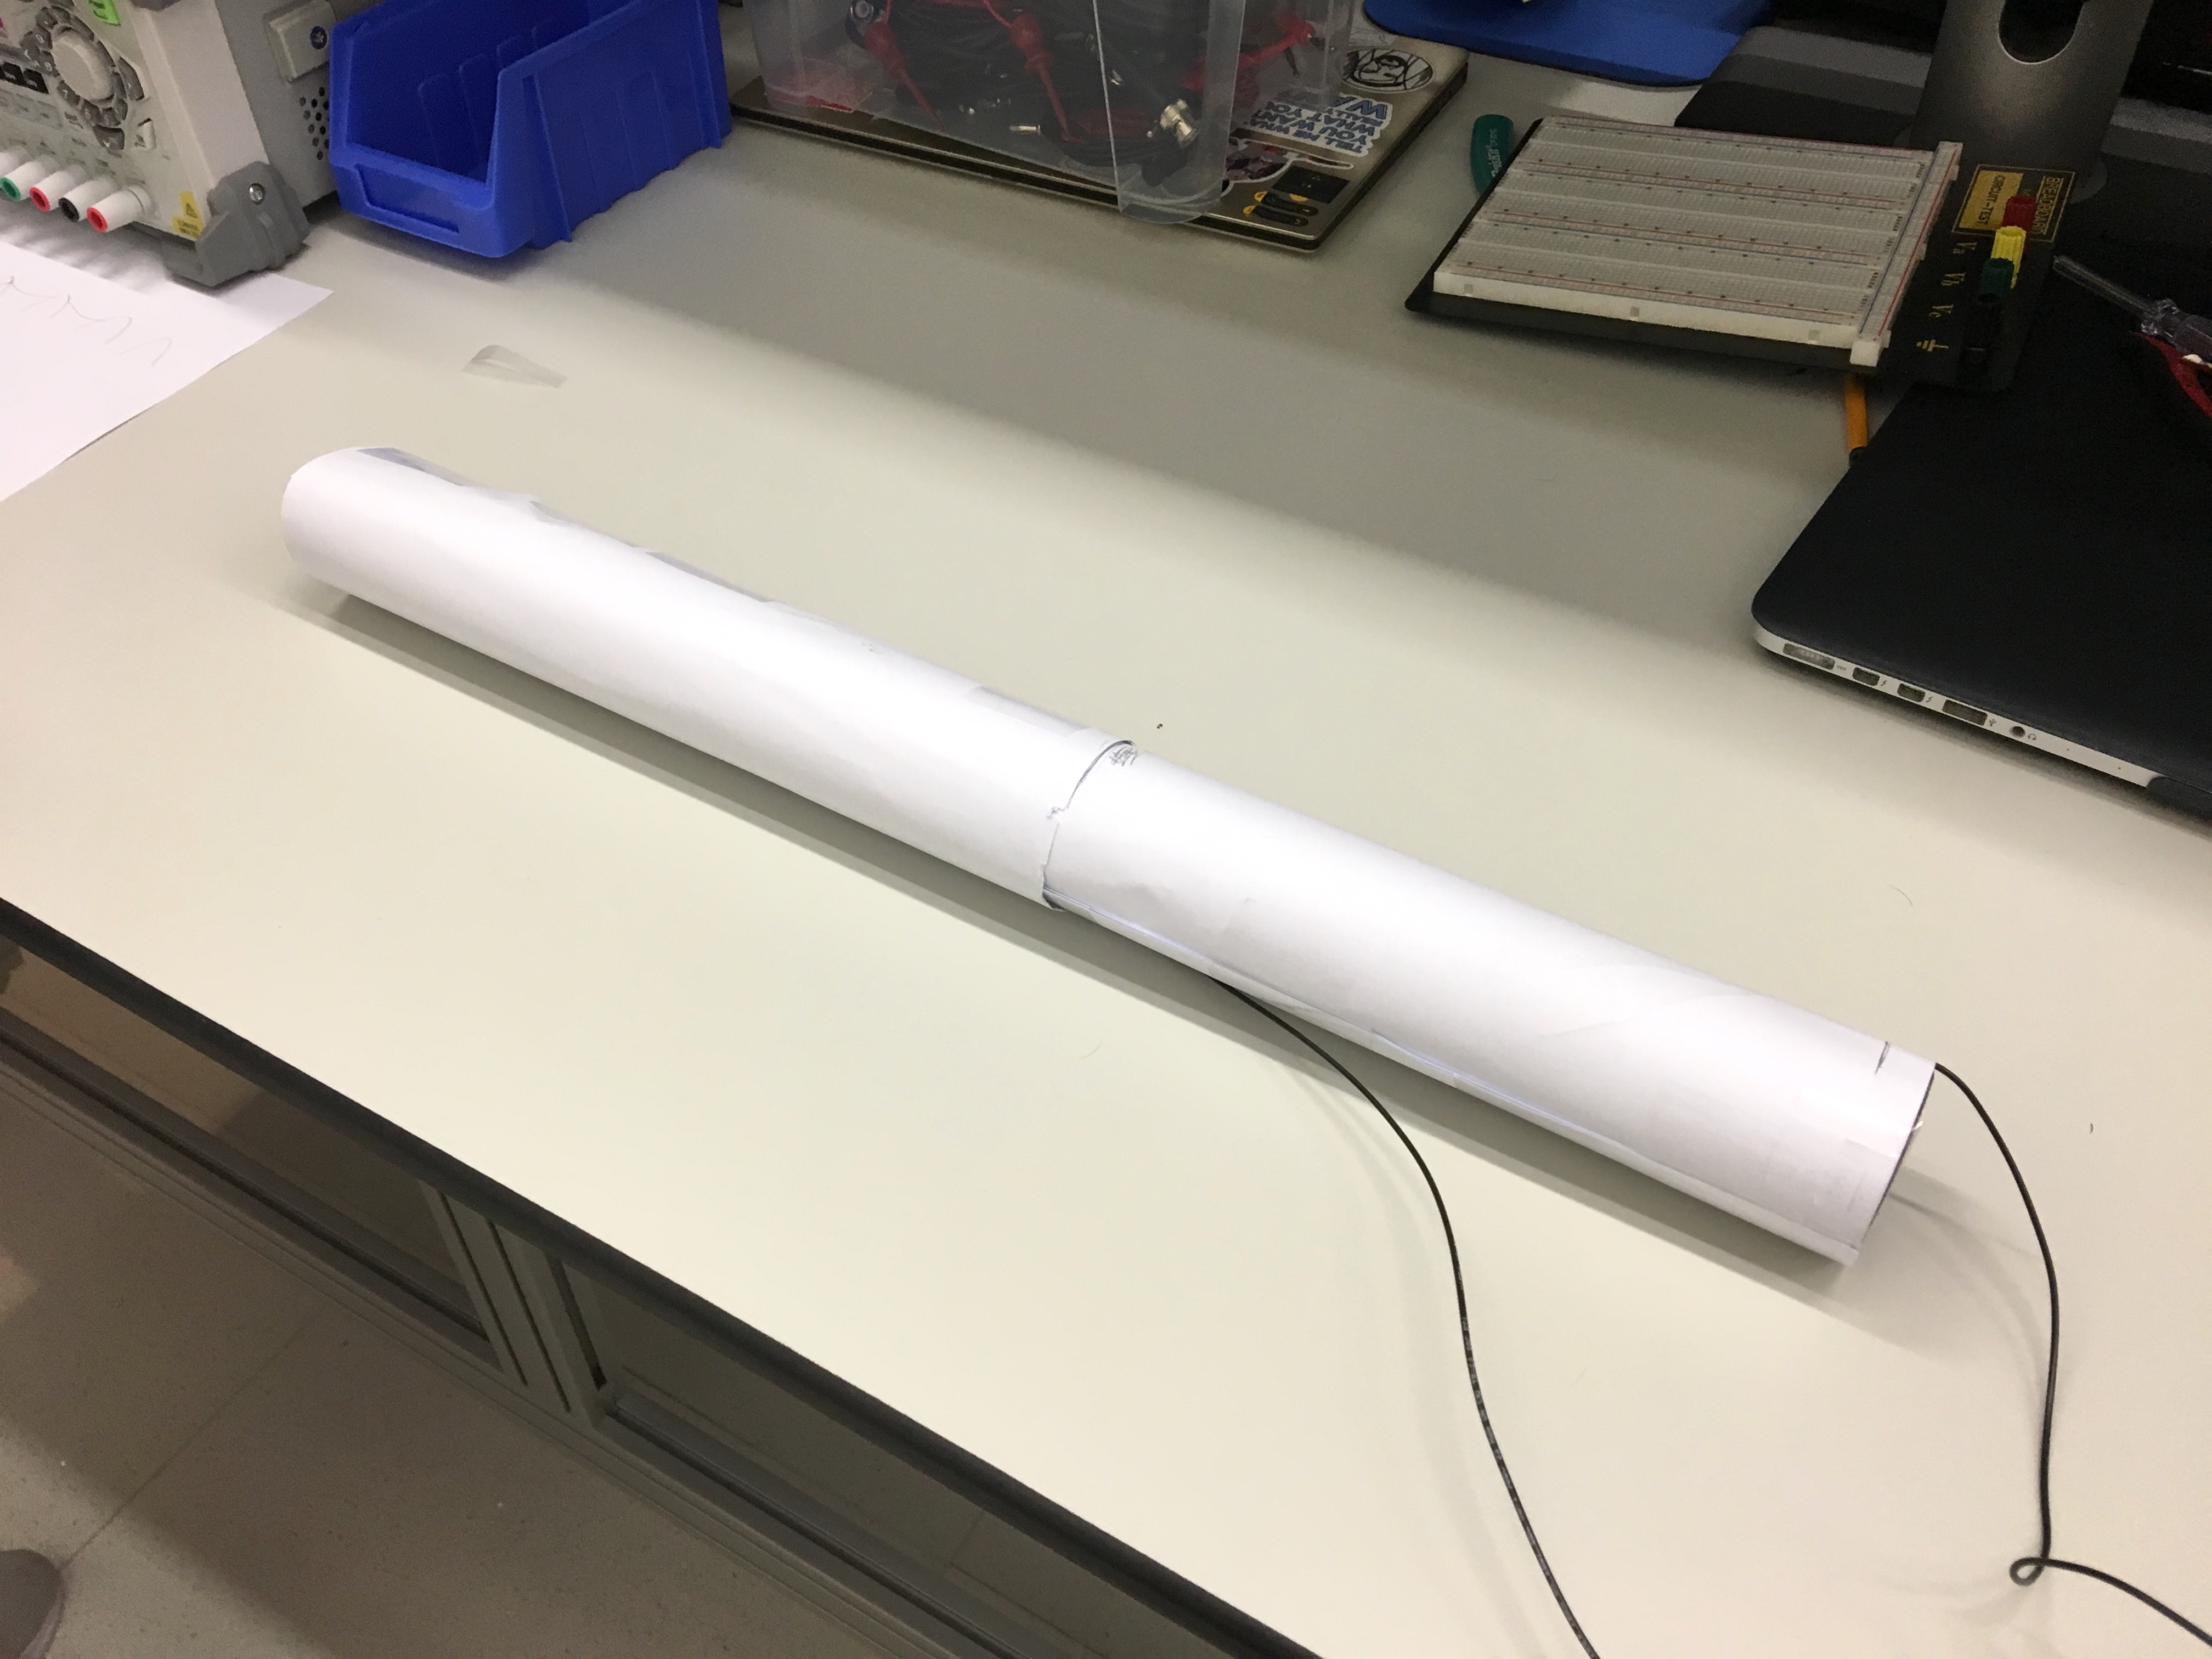
\includegraphics[width=\columnwidth]{images/lab4_3.jpg}
    \captionof{figure}{Variable capacitor at minimum capacitance }
    \label{fig:mincap}
    \medskip
\endgroup

\begingroup
    \medskip
    \centering
    %width=\columnwidth
    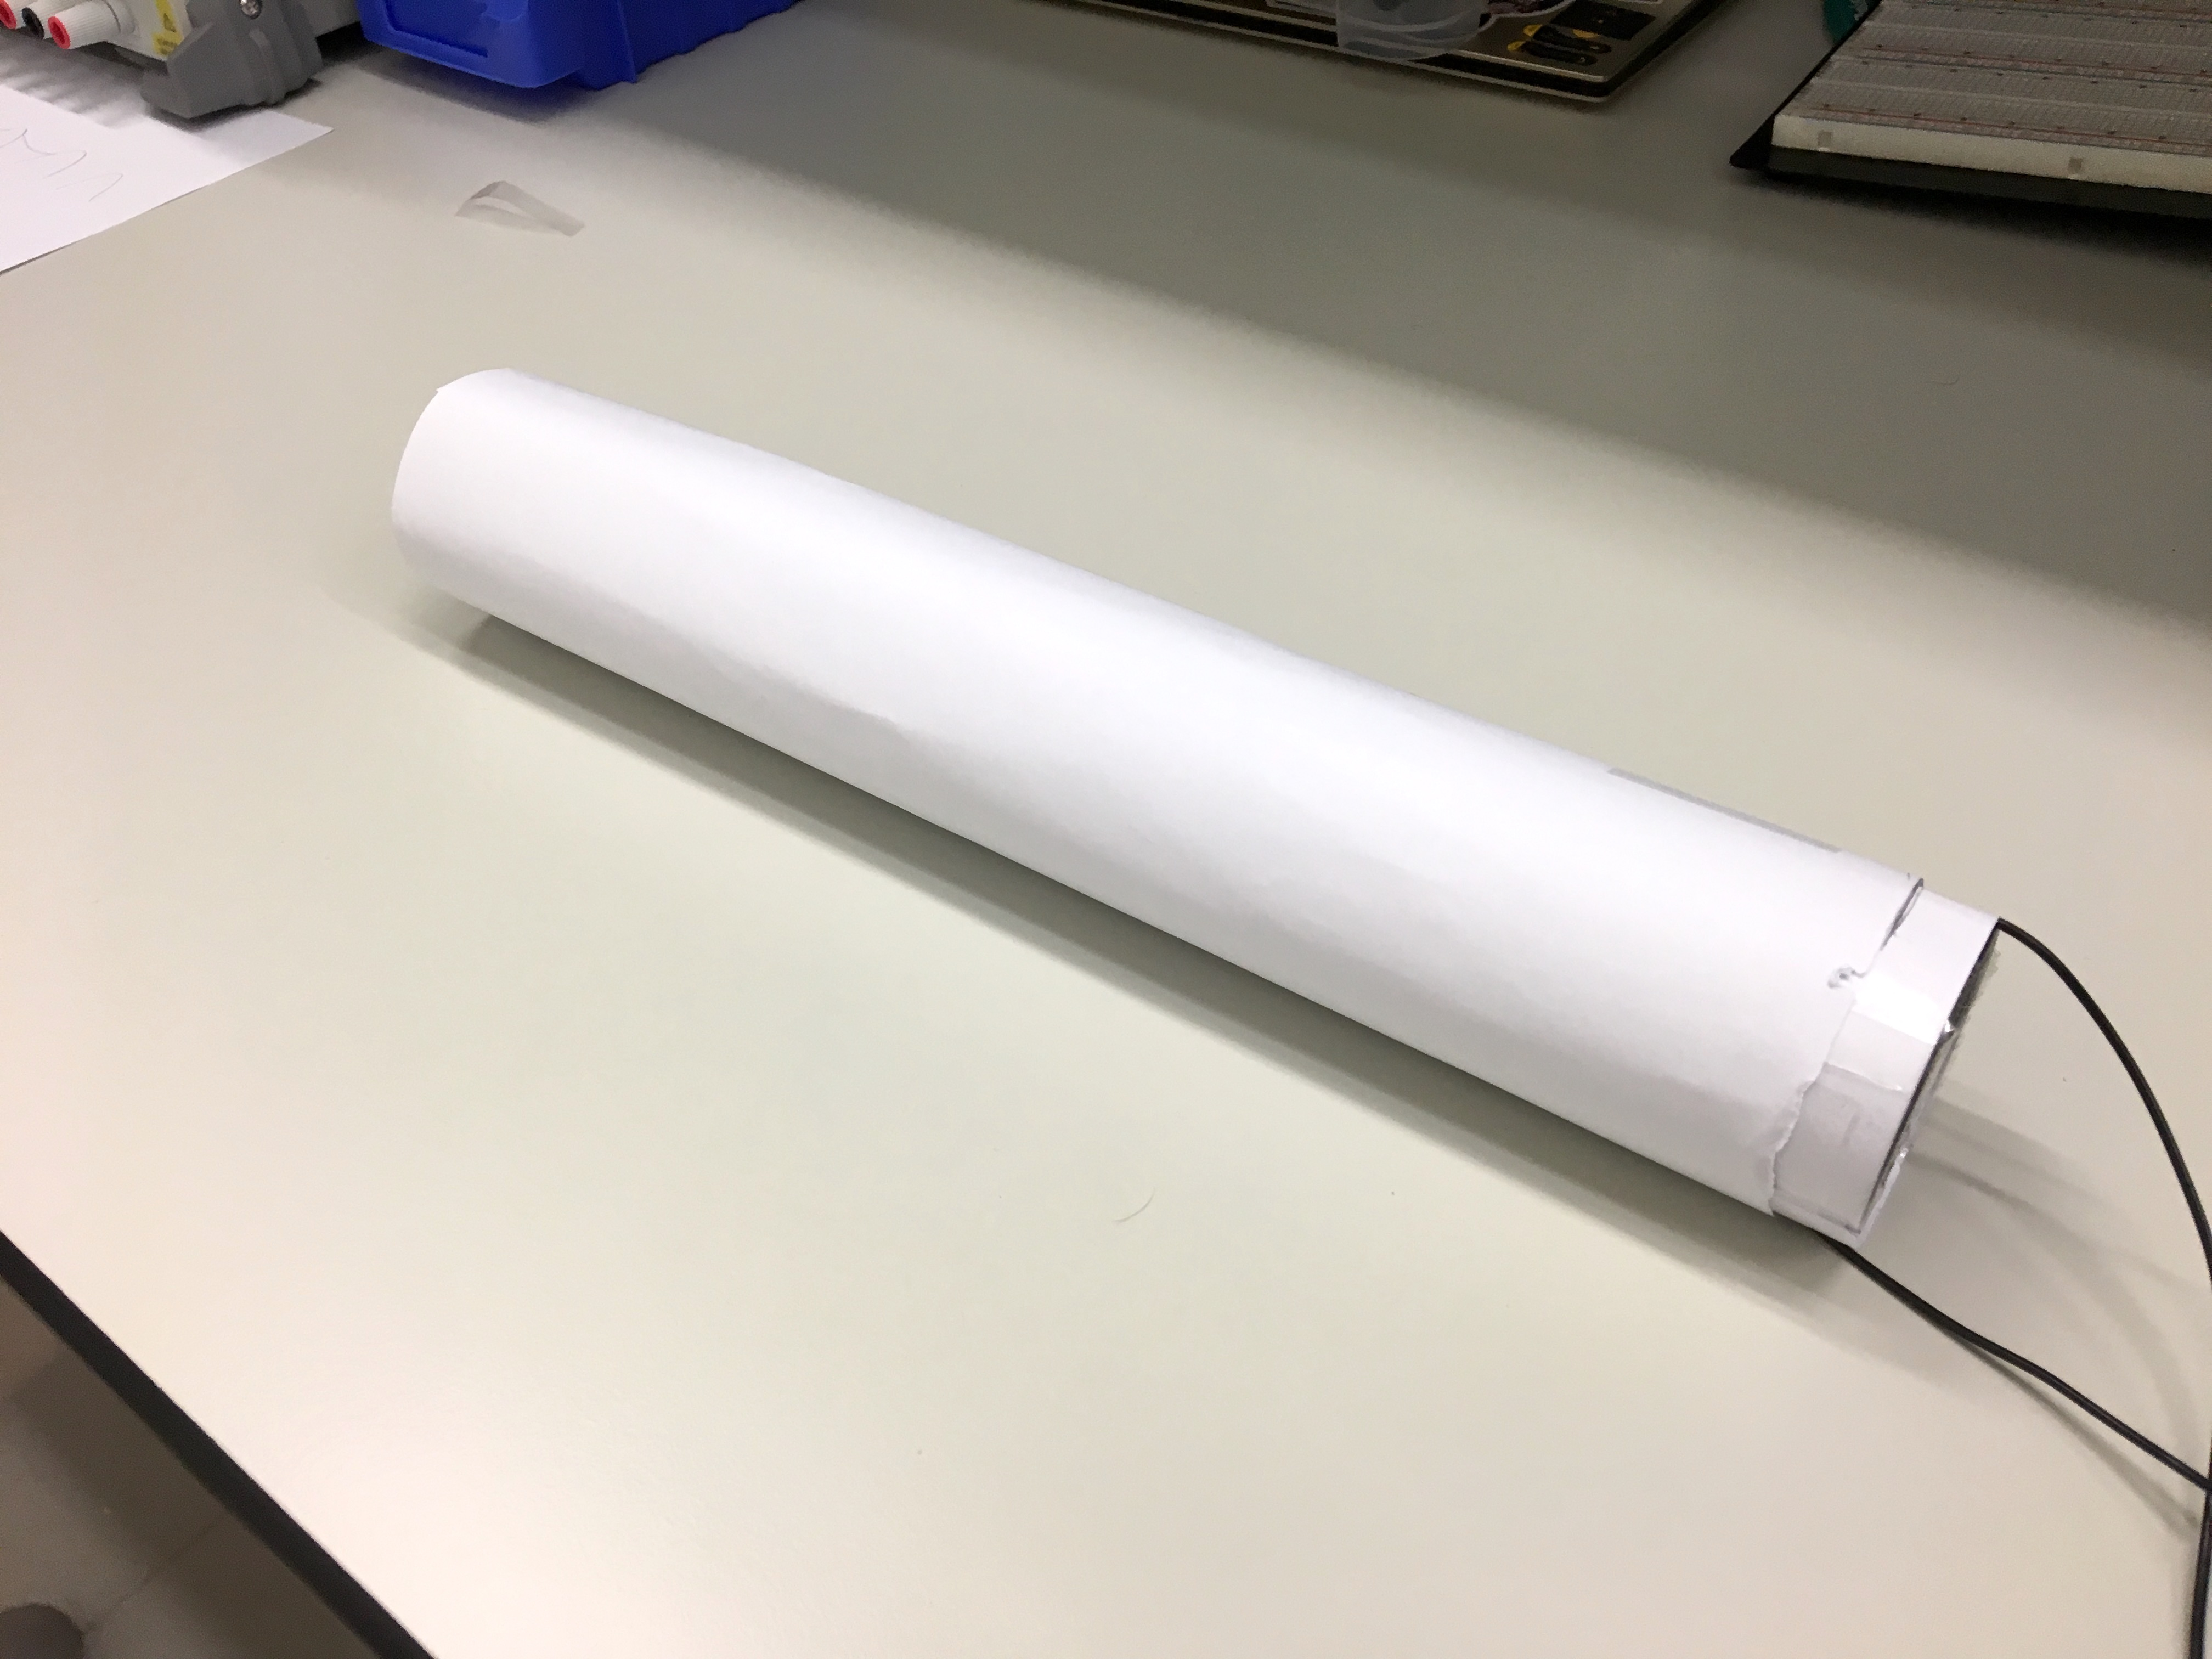
\includegraphics[width=\columnwidth]{images/lab4_4.jpg}
    \captionof{figure}{Variable capacitor at maximum capacitance}
    \label{fig:maxcap}
    \medskip
\endgroup

\section{Building the High-Pass and Low-Pass Filter Circuits}

\noindent Figures \ref{fig:HPF} and \ref{fig:LPF} show the circuit schematic for the produced HPF and LPF circuits. Furthermore, as a more practical representation, Figure \ref{fig:cad} approximately shows how the LPF circuit was implemented. 

\begingroup
    \medskip
    \centering
    %width=\columnwidth
    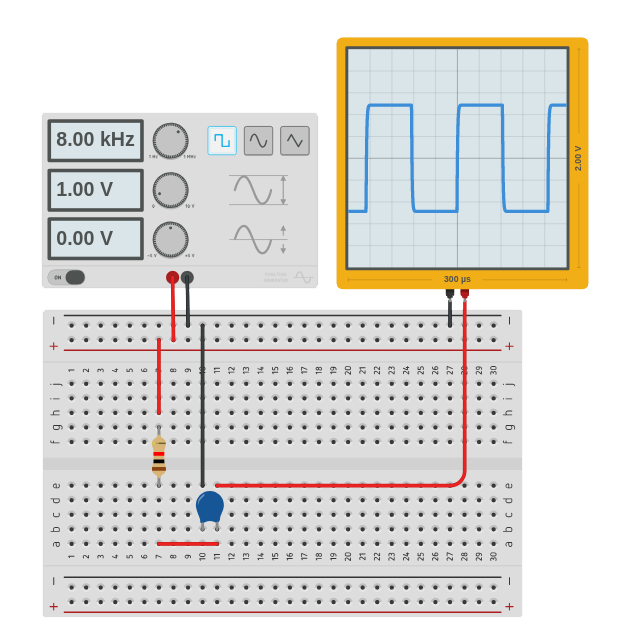
\includegraphics[width=\columnwidth]{images/lab4_7.png}
    \captionof{figure}{CAD representation of a LPF circuit}
    \label{fig:cad}
    \medskip
\endgroup

\noindent To build the LPF circuit, a BNC splitter was attached to the AC function generator. One of the outputs was connected directly to the oscilloscope, to visualize the voltage being supplied to the circuitry. The other output was connected directly to the resistor, which was connected in parallel with the capacitor. The voltage line of the circuit was finally connected to the oscilloscope, displaying the output voltage of the circuit. The LPF circuit operates on the principal that capacitors are reactive devices, acting as high resistance components to low frequency signals; therefore, low frequency signals pass almost directly to the oscilloscope, but a high frequency signal results in a much lower voltage output (see Figure \ref{fig:falstad1}).


\begingroup
    \medskip
    \centering
    %width=\columnwidth
    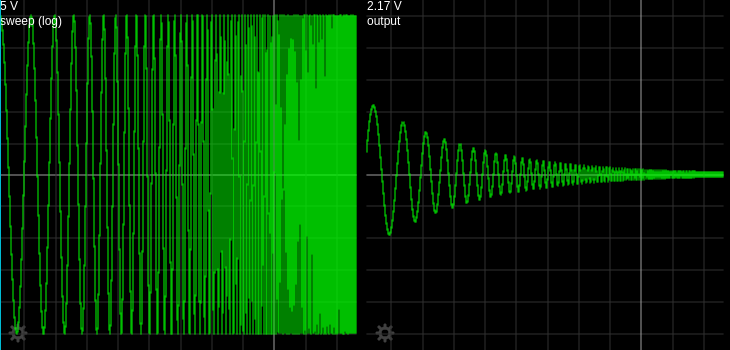
\includegraphics[width=\columnwidth]{images/lab4_8.png}
    \captionof{figure}{Voltage input and output depicting the operation of a LPF circuit}
    \label{fig:falstad1}
    \medskip
\endgroup

\noindent Similarly, to build the HPF circuit, the BNC splitter was utilized again to visualize input and output voltage. This time the capacitor was connected in series with the resistor. In this case, because capacitors act as high resistance towards low-frequency signals, only the high-frequency signals pass through the capacitor and thus reach the oscilloscope (see Figure \ref{fig:falstad2}.

\begingroup
    \medskip
    \centering
    %width=\columnwidth
    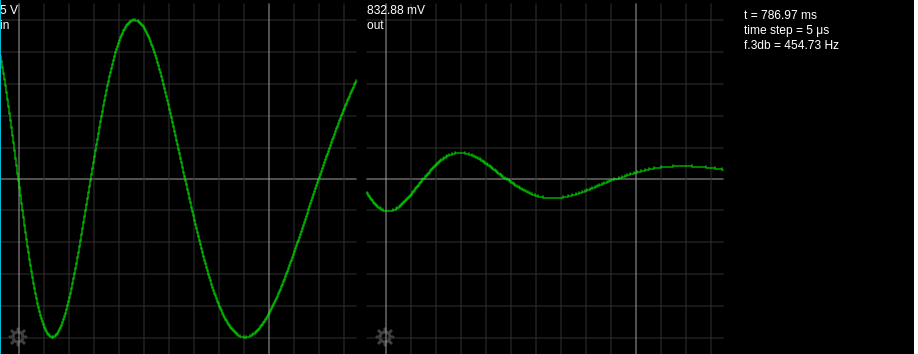
\includegraphics[width=\columnwidth]{images/lab4_9.png}
    \captionof{figure}{Voltage input and output depicting the operation of a HPF circuit}
    \label{fig:falstad2}
    \medskip
\endgroup


\smallskip
\section{Results}

\noindent As briefly explained, varying the frequency of the input voltage affects the output signal. The relation between the output and the input signal can be meaningfully described using gain, which is the ratio between the output voltage and the input voltage. Figure \ref{fig:tableLPF} and \ref{fig:tableHPF} represent the gain at varied frequencies at maximum capacitance, when the area shared between the two foil sheets was maximized. For the experiment, a $1V$ input signal was provided to both the HPF and LPF circuits. Therefore, the calculation of gain was simplified to just the output signal, as $\frac{x}{1} = x$ \\

\noindent The tables (see Figure \ref{fig:tableLPF} and \ref{fig:tableHPF}) support the claim that, for the HPF, as frequency increases the gain decreases. On the other hand, for the LPF, as frequency increases the gain increases. Furthermore, graphing the data (see Figure \ref{fig:graph1} and \ref{fig:graph2}) allows for visualizing the cutoff frequency of the two circuits. Cutoff frequency refers to the frequency at which the output signal is $\sqrt{\frac{1}{2}}$, approximately 0.707, of the input voltage within the passing band. The cutoff frequency is a tool used to label the boundary between the passband and stopband, therefore determining the operating range of the filtering circuit.\\

\begingroup
    \medskip
    \centering
    %width=\columnwidth
    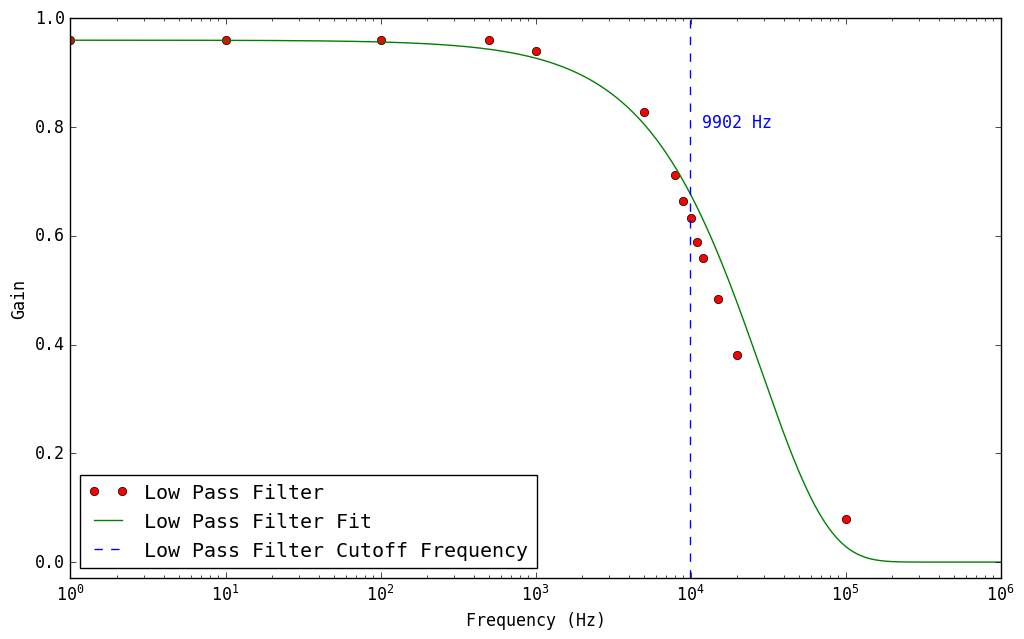
\includegraphics[width=\columnwidth]{images/lab4_11.png}
    \captionof{figure}{Plot of frequency against gain for the LPF circuit; the dashed blue line represents the cut-off frequency, representing the boundary frequency of the filtering circuit}
    \label{fig:graph1}
    \medskip
\endgroup

\begingroup
    \medskip
    \centering
    %width=\columnwidth
    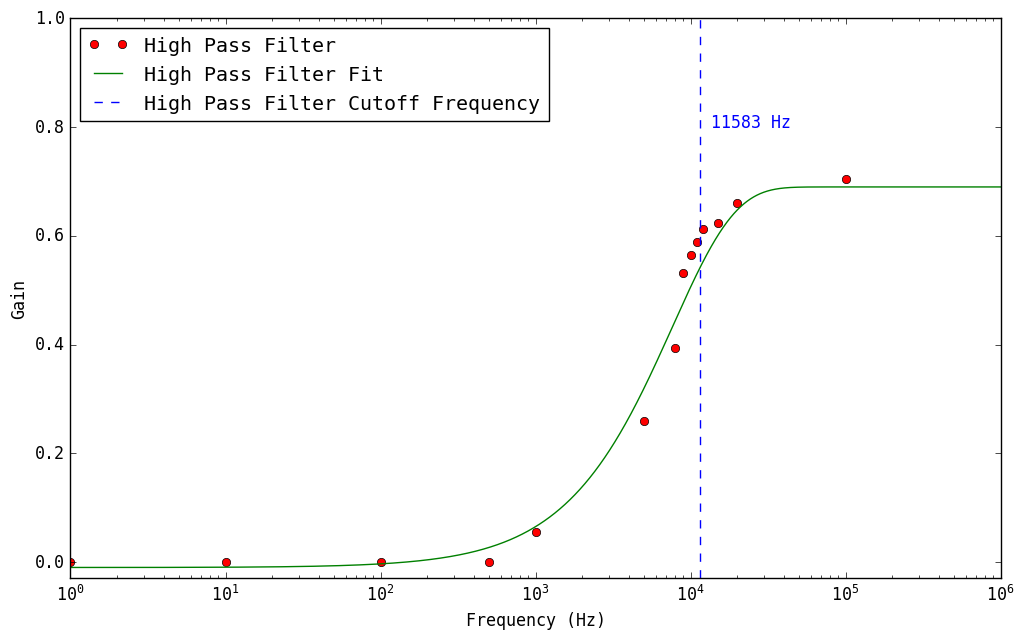
\includegraphics[width=\columnwidth]{images/lab4_10.png}
    \captionof{figure}{Plot of frequency against gain for the HPF circuit; the dashed blue line represents the cut-off frequency, representing the boundary frequency of the filtering circuit}
    \label{fig:graph2}
    \medskip
\endgroup

\noindent Graphing the data resulted in obtaining a best fit curve for both the circuits (see Equations \ref{eq:fitLPF} and \ref{eq:fitHPF}). The two fits were then solved for a y-value of $\sqrt{\frac{1}{2}}$ to obtain the cut-off frequencies. 


\begin{equation}
y = -0.7 \times e^{-7.0 \times 10^{-4} \times x ^{1.07}}+0.7
\label{eq:fitLPF}
\end{equation}


\begin{equation}
y = 0.96 \times e^{-3.5 \times {10^{-5}} \times x}
\label{eq:fitHPF}
\end{equation}

\noindent Determining the cutoff frequency therefore allowed for an approximation of the capacitance of the built capacitor, using the following formula (see Equation \ref{eq:cutoff}), where F is the cutoff frequency, R is the equivalent resistance, and C is the equivalent capacitance:

\begin{equation}
F = \frac{1}{2\pi RC}
\label{eq:cutoff}
\end{equation}

\begin{equation}
C = \frac{1}{2\pi RF}
\label{eq:cutoff}
\end{equation}



\noindent The table below (see Figure \ref{fig:tableCAP}) displays the calculated and measured capacitance of the built capacitor. The measured capacitance is well approximated by the experimental methods used to calculate the capacitance.  

\begingroup
    \medskip
    \centering
    \def\arraystretch{0.4}
    \begin{tabular}{lll}
\hline\\
& Low Pass Filter & High Pass Filter\\
\\
& (LPF) & (HPF) \\
\\
\hline
\\
F_{r} & 9982 Hz & 11583 Hz \\
\\
Max. CAP & 0.88 nF & 0.76 nF \\
\\
\hline
& & \\
\\
F_{r} & 19145 Hz & N/A \\
\\
Min. CAP & 0.46 nF & N/A \\
\\
\hline
\\
& & \\
Measured Max. & \multicolumn{2}{c}{ 0.82 nF } \\
\\
Measured Min.& \multicolumn{2}{c}{ 0.33 nF } \\
\\
\hline
\end{tabular}
    \captionof{figure}{Tabulation of the gain against varied frequency of the input voltage (Hz) at max capacitance for LPF}
    \label{fig:tableCAP}
    \medskip
\endgroup

\begingroup
    \medskip
    \centering
    \def\arraystretch{1.5}
    \begin{tabular}{cc}
    \hline
    Frequency (Hz) & Gain \\
    \hline
    1 & 0.960 \\
    10 & 0.960 \\
    100 & 0.960 \\
    500 & 0.960 \\
    1k & 0.940 \\
    5k & 0.828 \\
    8k & 0.712 \\
    9k & 0.664 \\
    10k & 0.632 \\
    11k & 0.588 \\
    12k & 0.560 \\
    15k & 0.484 \\
    20k & 0.380 \\
    100k & 0.080 \\
    1000k & 0.011 \\
    \hline
    \end{tabular}
    \captionof{figure}{Tabulation of the gain against varied frequency of the input voltage (Hz) at max capacitance for LPF}
    \label{fig:tableLPF}
    \medskip
\endgroup

\vspace{15mm}

\begingroup
    \medskip
    \centering
    \def\arraystretch{1.5}
    \begin{tabular}{cc}
    \hline
    Frequency (Hz) & Gain (mV) \\
    \hline
    1 & 0 \\
    10 & 0 \\
    100 & 0 \\
    500 & 0 \\
    1k & 56 \\
    5k & 260 \\
    8k & 394 \\
    9k & 532 \\
    10k & 564 \\
    11k & 588 \\
    12k & 612 \\
    15k & 624 \\
    20k & 660 \\
    100k & 704 \\
    1000k & 768 \\
    \hline
    \end{tabular}
    \captionof{figure}{Tabulation of the gain against varied frequency of the input voltage (Hz) at max capacitance for HPF}
    \label{fig:tableHPF}
    \medskip
\endgroup

\noindent Furthermore, Figures \ref{fig:square1} and \ref{fig:square2} show the result of applying a square wave input on the LPF and HPF. The green wave forms shown on the screen of the oscillator are the original square wave forms generated by the waveform generator. However, the yellow forms are showing how HPF and LPF modify the waves. The curves shown in the yellow waveform is caused by the discharge and charge period of the capacitor. The frequency of the generated square waveform is slow enough that the connected capacitor can have enough time to charge & discharge and this is reflected the voltage levels shown in the oscilloscope.

\begingroup
    \medskip
    \centering
    %width=\columnwidth
    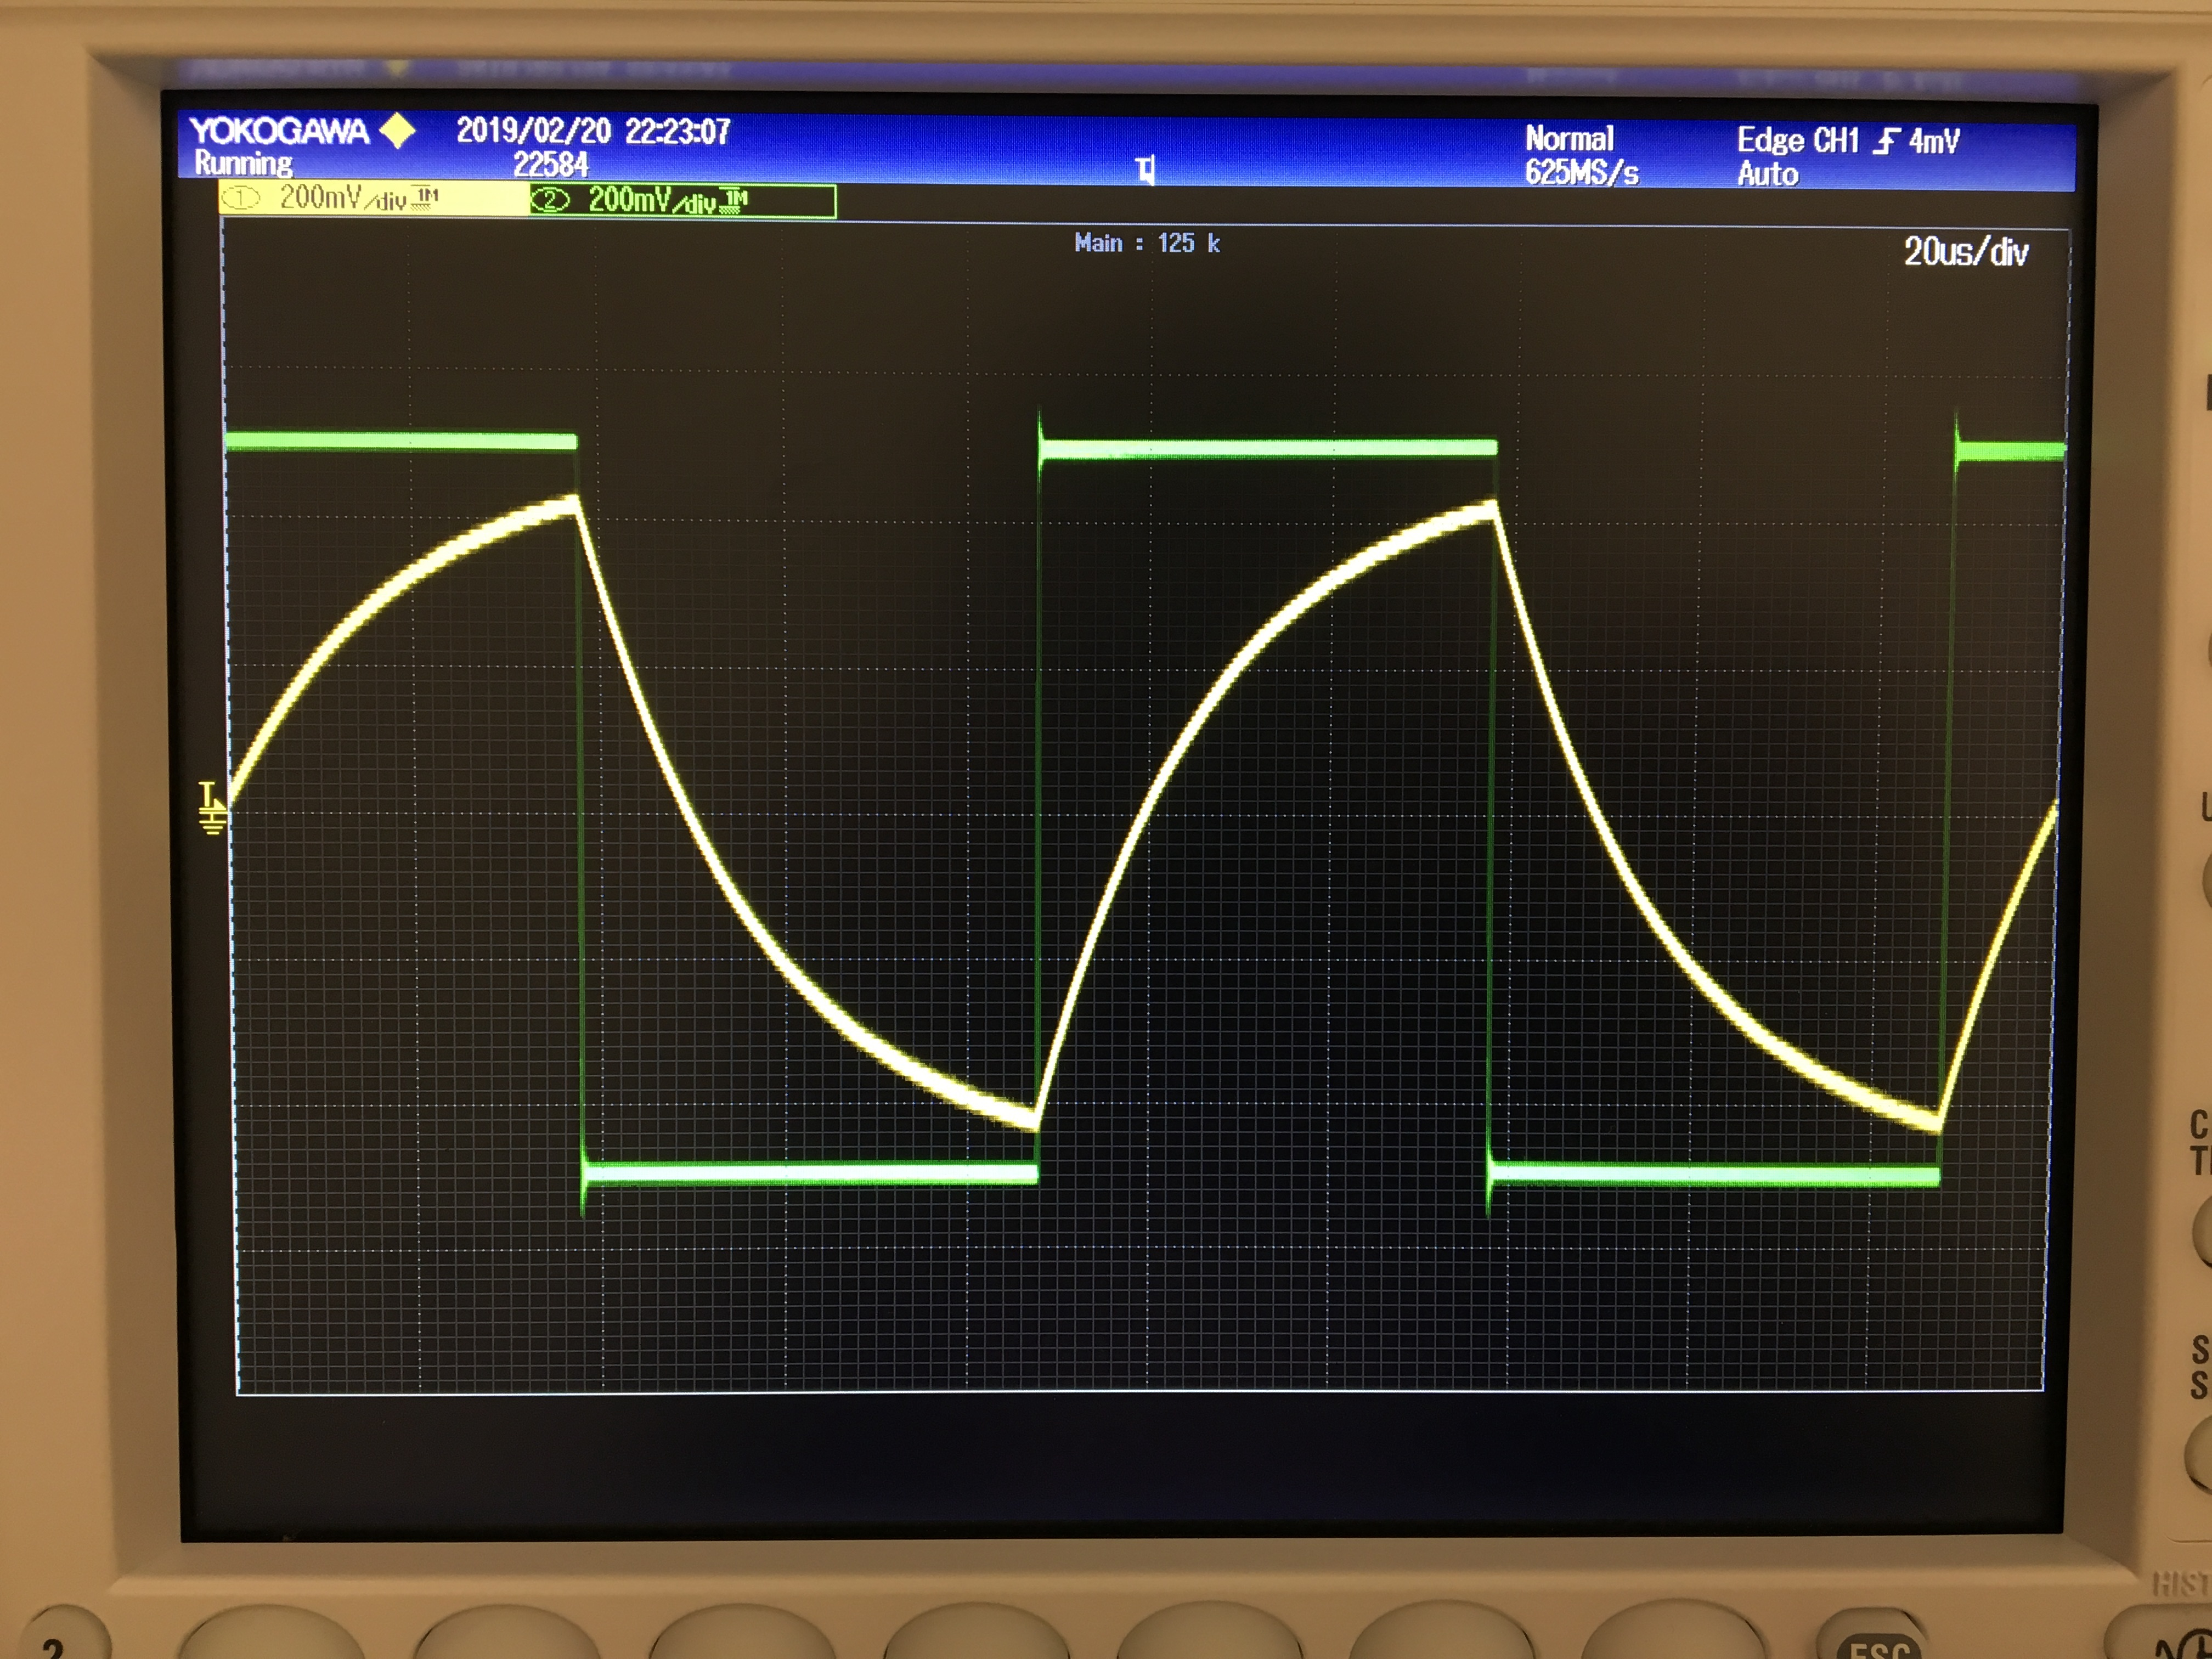
\includegraphics[width=\columnwidth]{images/lab4_1.jpg}
    \captionof{figure}{Applying a square wave to the LPF circuit at 10KHz}
    \label{fig:square1}
    \medskip
\endgroup


\begingroup
    \medskip
    \centering
    %width=\columnwidth
    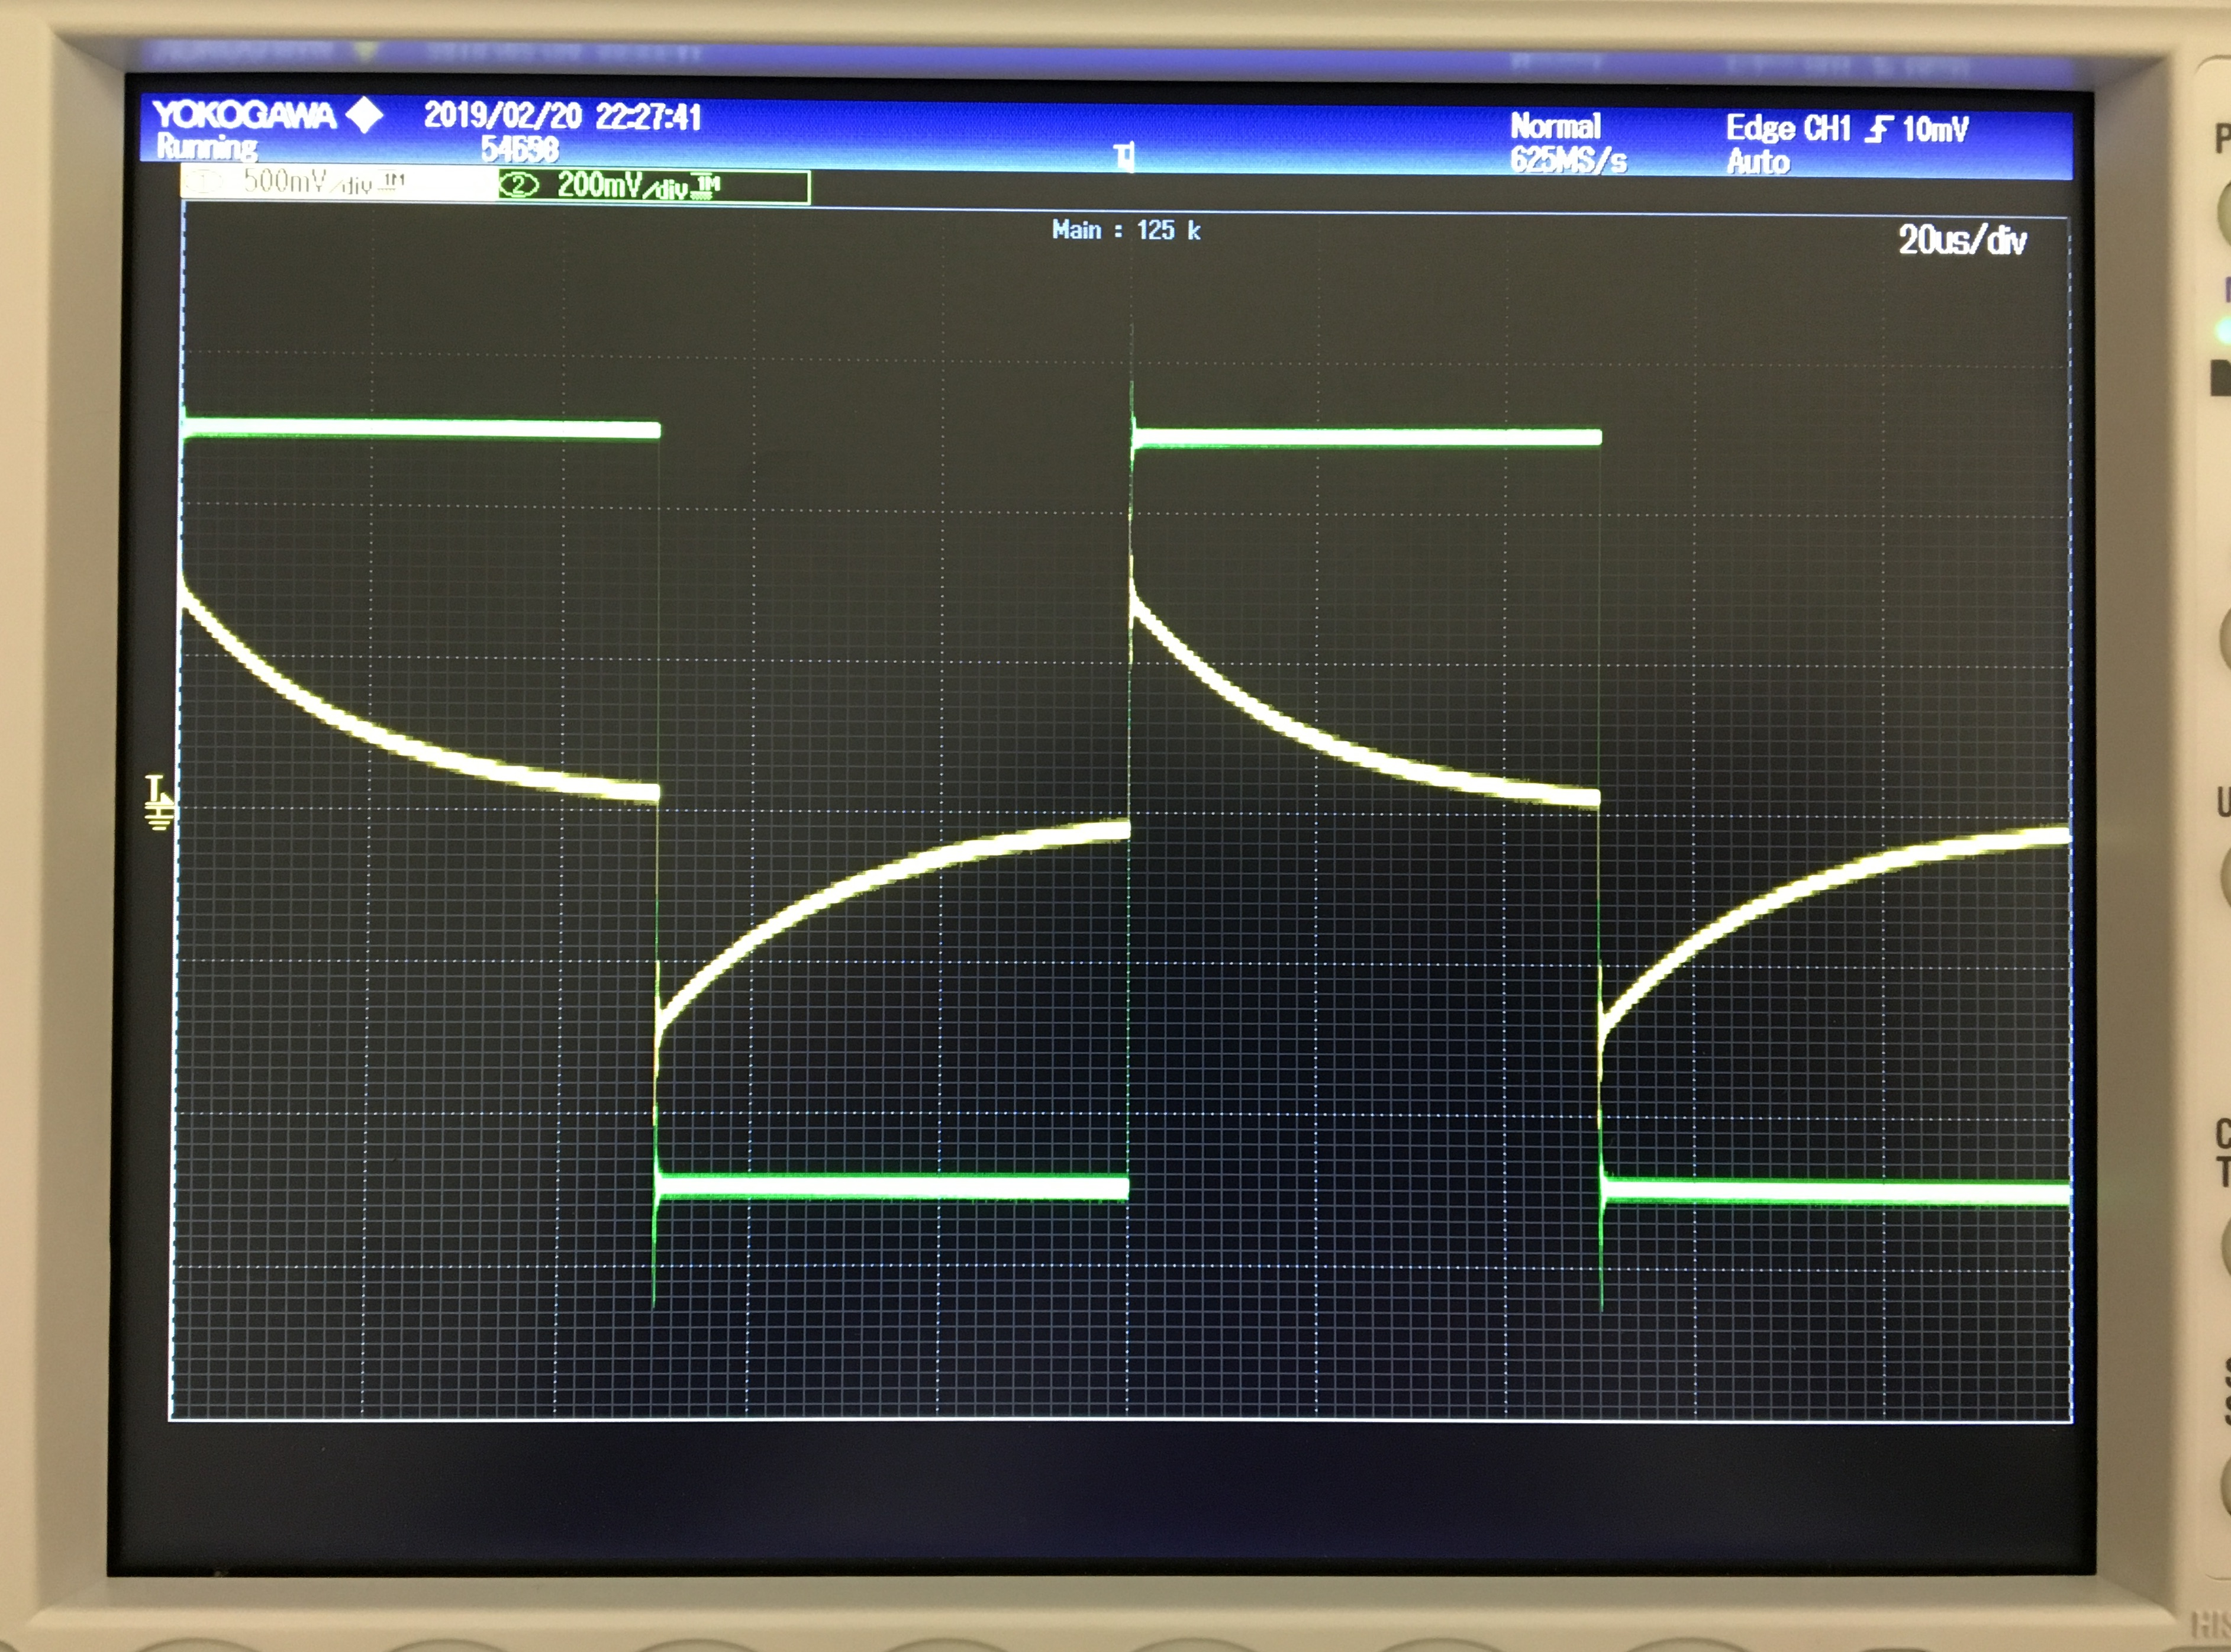
\includegraphics[width=\columnwidth]{images/lab4_2.jpg}
    \captionof{figure}{Voltage input and output depicting the operation of a HPF circuit}
    \label{fig:square2}
    \medskip
\endgroup


% \begingroup
%      \medskip
%      \centering
%      %width=\columnwidth
%      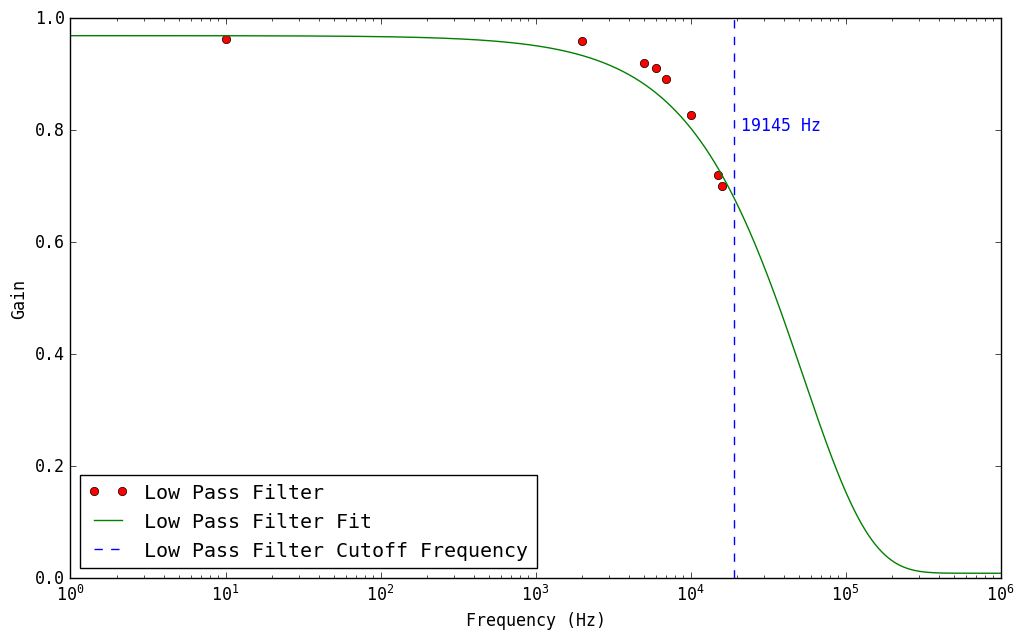
\includegraphics[width=\columnwidth]{images/lab4_12.png}
%      \captionof{figure}{CMIN}
%      \label{fig:square2}
%      \medskip
%  \endgroup


\smallskip
\section{Conclusions}

\noindent A capacitor was built using aluminum foil as the conducting material and paper as a dielectric. The capacitor was then used to build HPF and LPF circuits, where a $1V$ input signal was applied across both circuits. Varying the frequency of the input signal and measuring the output voltage allowed for the measurement of gain. Graphing this data and applying an exponential fit led to the cut-off frequency of the two filtering circuits. The cutoff frequency ($F_{r}$) for the LPF circuit was approximately $9982 Hz$ at maximum capacitance, resulting in a calculated value of 0.88 nF. On the other hand, the $F_{r}$ for the HPF circuit was approximately $11583 Hz$, resulting in a calculated value of 0.76 nF. When measured using a LCR meter, the maximum capacitance was 0.82 nF, falling within the calculated range. Similarly, the minimum capacitance was calculated to be approximately 0.46 nF and was measured to be 0.33 nF.\\

\noindent This experiment determined that manipulating the formula for cut-off frequency is a valid method to calculate an unknown capacitance; furthermore, this experiment may have been extended to similarly calculate the unknown resistance of a filtering circuit. The experiment also depicted how a given capacitor, when placed in a deliberate way, filtered different frequencies, resulting in cutoff frequencies in a similar region. Therefore, this quality could be exploited to merge a HPF and LPF circuit to produce a band pass filter (BPF), which would allow for a very narrow band of frequencies to pass through. BPF are crucial to wireless communications, where transmitters are allocated a certain frequency range. Thus, producing and detecting an output signal within a certain band assures that the communication does not interfere with other transmitters with their alloted frequency bands. These devices can be used in wide variety of devices for communication such as AM/FM radios, cell phone, satellite, etc.




%\appendices
%\section{Proof of the First Zonklar Equation}
%Appendix one text goes here.

%\section*{Acknowledgment}

\printbibliography

\end{document}